\chapter{Proceso de aprendizaje}

Tras las descripción de los modelos a utilizar, y las funciones de pérdida a emplear, comienza el proceso de entrenamiento de los modelos. Este proceso es uno de los más lentos de todo el desarrollo del proyecto, debido a la cantidad de horas necesarias a esperar para recopilar los resultados del modelo. Se estudiará la eficiacia de cada modelo a la hora de evaluar el problema, y las decisiones tomadas para su mejora y elección.\\

Para resolver este problema, se ha tomado un enfoque de dos niveles; en primer lugar, distinguiremos si la enfermedad que se recibe como entrada se trata de un ejemplar de enfermedad maligna o benigna, y posteriormente, su salida indicará un segundo modelo a aplicar sobre la enfermedad, especializado únicamente en uno de los dos tipos de enfermedades. Así, conseguimos un conjunto de modelos especialziados que permiten otorgar el diagnóstico con mayor precisión y seguridad.\\

Un aspecto clave de este proceso será la eficiencia, pero sobre todo el correcto diagnóstico de las enfermedades, por lo que usaremos como métricas de selección la precisión, el recall y el accuracy balanceado:

\begin{itemize}
	\item Precision = TP / (TP + FP). Proporción de valores bien clasificados dentro de una clase teniendo en cuenta verdaderos y falsos positivos.
	\item Recall = TP / P. Valores correctamente identificados como positivos respecto al total de elementos positivos.
	\item Accuracy balanceado: combina sensitivity (TP/(TP+FN)) y specificity (TN/(TN+FP)). La primera, devuelve el valor real de proporción de valores correctamente clasificados entre el total de casos positivos que tenemos (contando predicciones positivas y falsos negativos), mientras que la especifidad, nide el caso dual: la proporción de casos negativos bien clasificados respecto al total de datos negativos tanto bien clasificados como mal clasificados, y que son identificados como falsos positivos. Esto nos permite calcular el accuracy de forma proporcional al porcentaje de presencia de las clases, e intentamos así paliar el efecto del desequilibrio de los datos:
	
$$ Balanced\ accuracy: \frac{Sensitivity + Specificity}{2}$$
	
	En base a esta expresión, podemos saber que si el valor es aproximadamente 1/númeroClases, es posible que gran parte de las clases no estén siendo correctamente clasificadas en caso de ser minoritarias. Valores mayores nos harán conocer que el resultado de clasificar todas las clases es satisfactorio.
\end{itemize}

\section{Clasificación binaria}

El problema de la clasificación binaria consiste en la distinción de las enfermedades malignas de aquellas que son benignas. Se trata del primer problema a resolver antes de especificar el tipo de enfermedad que posee el paciente, y así poder especializar los modelos segundo nivel.

\subsection{Equilibrio de los datos}

El primer inconveniente que nos encontramos para este problema es el inmenso desbalaceo entre la clase benigna y maligna. Si redibujamos el gráfico mostrado durante la fase de preprocesamiento de datos, únicamente con los datos de entrenamiento, obtenemos lo siguiente: 

\begin{figure}[H]
	\centering
	\label {desequilibriototal}
	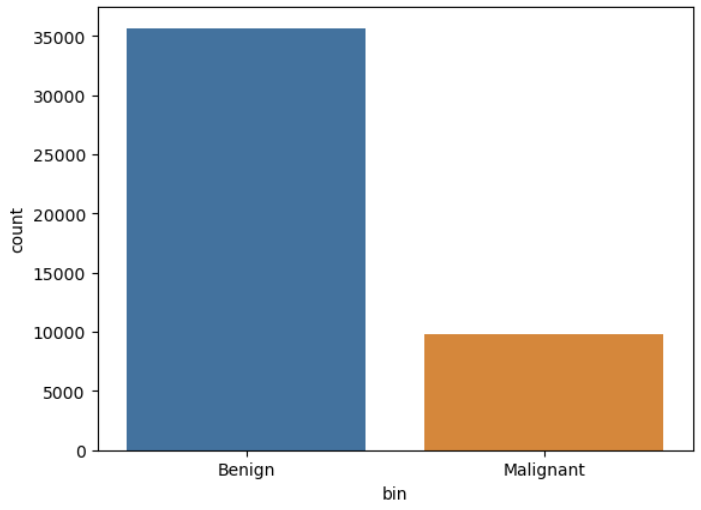
\includegraphics[scale = 0.4]{imagenes/desequilibriototal.png}
	\caption{Desequilibrio de datos}
\end{figure}

Se puede observar la alta disparidad existente entre ambas, siendo 35664 casos benignos y 9752 malignos. Es una diferencia de 3.65 veces más casos benignos que malignos, lo que se traduce en un equilibrio de  79\% y 21\% respectivamente. Para paliarlo, podemos efectuar dos estrategias: aplicar técnicas de oversampling (también conocido como sobremuestreo sintético), donwsampling de la clase mayoritaria, o bien, la aplicación de penalziaciones sobre la clase minoritaria para que su incorrecta clasificación tenga mayores consecuencias (haciendo uso de FocalLoss).\\

\subsubsection{Técnicas descartadas}

La ténica de downsampling de la clase mayoritaria queda descartada, debido a que dentro de esa clase, podemos encontrar etiquetas de segundo nivel asociadas a las enfermedades que se pueden diagnosticar. Como algunas de estas clases son muy escasas en número, si realizamos downsampling de forma aleatoria sin ningún tipo de restriccióin, podría darse el caso límite en la que una clase completa desapareciese del cojunto. Y esto conllevaría a la obtención de errores al evaluación de test, pues tendríamos una clase presente en test no estudiada en entrenamiento, que sólo provocaría un aumento de las métricas de error. \\

El uso de la función de pérdida FocalLoss podría ayudar a paliar este efecto. Sin embargo, debido al desajuste 79-21 del que disponemos, y la gran variedad de imágenes, se trata de una solución demasiado arriesgada. Para comprobarlo, se sometíó a evaluación con los valores por defecto recomendados de Resnet50. A priori, los resultados podrían parecer correctos en validación \ref{tab:resultsfl}; sin embargo, observamos que la clase minoritaria, la maligna, obtiene resultados que no están a la altura de la clase mayoritaria. Observamos un valor 0.41 en recall, valor preocupante frente al 0.95 de la clase benigna. Al existir un recall bajo, quiere decir que esta clase no se está detectando adecuadamente como maligna, y casi el 60\% de sus casos son calificados como benignos. Esto es un grave problema, ya que los casos malignos son los que más riesgo conllevan para la salud. Por tanto, se descarta también esta estrategia.


\begin{table}[!ht]
	\centering
	\begin{tabular}{|l|c|c|c|c|}
		\hline
		& Precision & Recall & F1-score & Support \\
		\hline
		Benign & 0.86 & 0.95 & 0.90 & 15338 \\
		Malignant & 0.68 & 0.41 & 0.51 & 4126 \\
		\hline
		Accuracy &  &  & 0.83 & 19464 \\
		Macro avg & 0.77& 0.68& 0.71&19464\\
		Weighted avg&0.82&0.83&0.82&19464\\
		\hline
	\end{tabular}
	\caption{Informe de clasificación}
	\label{tab:resultsfl}
\end{table}

\subsubsection{Propuesta: oversampling}

Sólo nos queda disponible la estategia de oversampling: la ampliación sintética de la clase minoritaria. Este proceso es muy delicado, ya que se basa en realizar alteraciones sobre las imágenes disponibles para dotarlas al conjunto de una mayor variabilidad, hasta equiparar el número de ejemplares con el de la clase mayoritaria. Existen distintas técnicas a aplicar, pero en este caso, utilizaré la estrategia de realizar alteraciones sobre las imágenes mediante una biblioteca de transformaciones: imgaug.

Se aplicarán una serie de transformaciones la imagen que alteren su estructura, pero con cuidado de no generar imágenes demasiado modificadas que se alejen de la distribución original de la clase maligna. Para realizar las transformaciones, he contruido un pipeline, una secuencia de transformaciones que aplica, en orden aleatorio, y con cierta probabilidad, las siguientes variaciones:

\begin{itemize}
	\item Fliplr(p=0.5). Se trata de un efecto de espejo de la imagen, respecto a su eje horizontal. Es equivalente a realizar una rotación de la imagen de 180º sobre su eje teórico horizontal que transcurre por la mitad de la imagen. Esta alteración se realziará con un 50\% de probabilidad.
	\item Flipud(p=0.5). Se trata de un efecto de espejo de la imagen, respecto a su eje vertical. Es un caso de efectos similares al anterior, aplicado con un 50\% de probabilidad.
	\item Gaussian blur (p=0.5). Se aplicará filtro gaussiano en el 50\% de los casos, especificándose un valor de sigma muy pequeño de 0.5.
	\item Modificación de contraste  (p=0.25). Se aplicará un aumento o decremento del contraste del 20\% en el 25\% de los casos. Esto emula posibles cambios de luminosidad ambiente y de profundidad de color de la cámara
	\item Ruido Gaussiano aditivo  (p=0.5). Se aplica en caso de que el ruido gaussiano estándar no sea aplicado. Aplica un filtro gaussiano a nivel de canal, de forma que solo parte de la imagen se encuentra difuminada.  Se aplica también en un 50\% de los casos
	\item Transformaciones afines  (p=0.2): se trata de una alteración compuesta de escala y zoom, y una posterior traslación o rotación de la imagen. Se trata de una opcionalidad ofrecida por imgaug de forma no configurable directamente.
\end{itemize}

Estos valores han sido escogidos tomando como inspiración las transformaciones realizadas por el equipo ganador de la competición de ISIC \cite{1stISIC}, debido a sus buenos resultados.

Es importante destacar que dichas transformaciones únicamente se han realizado sobre los datos de entrenamiento; los datos de validación y test permanecen inalterados de forma que éstos sigan siendo un estimador no sesgado del rendimiento del modelo. Poir tanto, la extracción del 30\% de validación se realiza antes del sobremuestreom y los dos subconjuntos se guardan en carpetas distintas, a las que llamaremos train y test.

\subsection{Construcción del modelo}

Con los datos preparados, configurar mediante Fastai y Pytorch los modelos que deseamos probar. Los 3 modelos siguen la misma configuración, a excepción de la importación del modelo, por lo  que será explicado de forma paramétrica. Tenemos 3 tareas diferenciables: la creación del datablock para la gestión de los datos, el entrenamiento del modelo, y la transformación del mismo al modelo cuantizado empleado en el dispositivo Android.

\subsubsection{Creación del datablock}

FastAI ofrece el tipo de objeto Datablock para la creación de una estructura que organiza los datos de entrenamiento. Permite construir un bloque con todos los datos, de forma que cualquier consulta o verificación pueda realizarse sobre un mismo objeto. Consta de varios parámetros que podemos ajustar para normalizar las imágenes, adaptar el tamaño de entrada, o realizar la separación train-validación. Desglosadando los parámetros más importantes, tenemos:

\begin{itemize}
	\item blocks. Nos permite establecer el formato de entrada de datos, y la salida que queremos obtener de los mismos. En problemas de clasificación, habitualmente, tendremos como entrada un bloque de imágenes, y como salida, queremos obtener un conjunto de categorías asociados al bloque.
	\item get\_items. Establece la fuente de la cual obtener los datos para la construcción del DataBlock. Se trata de una función preconfigurada para la lectura de datos dado un repositorio o dirección de disco. En nuestro caso, como las imágenes no contienen información compleja, como plantillas de segmentación, se importan directamente de esta forma.
	\item splitter. Permite especificar divisiones de los datos. Habitualmente, se utiliza la función RandomSplitter, que nos permite separar los datos en entrenamiento y validación. Como parámetros de entrada, recibe el porcentaje de datos para validación que queremos obtener, y opcionalmente una semilla, por si deseamos repetibilidad de los experimentos. Como en este caso, queremos que el conjunto de entrenamiento sea el conjunto sobremuestreado, y validación, sea la carpeta valid, se ha creado una función que indica 1 si la imagen pertenece a la carpeta valid, y 0, si se encuentra en train. \ref{fig:particiones}
	\item get\_y. Parámetro al cual se asocian las etiquetas de los elementos de entrada. Puede recibir una función o bien una lista con las etiquetas asociadas a los elementos del dataset. FastAI toma las etiquetas por defecto del nombre de carpeta, por lo que tendremos que especificarle una función que tome la etiqueta del dataset \ref{fig:etiquetadobinario}.
	\item item\_tfms. Establece modificaciones sobre las imágenes de forma previa a la ejecución del modelo. En este caso, como ya hemos realizado oversampling, no realizaremos ninguna otra modificación sobre las imágenes para no transformar en exceso los datos.
	\item batch\_tfms. Permite realizar transformaciones a nivel de batch. Permite aplicar operaciones como la normalización de las imágenes. Este procedimiento favorece la convergencia del modelo, aunque el cálculo de la media y desviación típica es costoso. En su lugar, utilizaré la normalización que provee ImageNet, donde ya se incluyen los valores estadísticos de media y desviación para los datos en la variable *image\_stats provenientes de decenas de millones de imágenes.
	
\end{itemize}


 \begin{algorithm}[H]
	\caption{Función para la distinción de entrenamiento y validación}
	\label{fig:particiones}
	\begin{algorithmic}[1]
		
		\Procedure{ val\_splitter}{fname}
		\Comment{Comprueba si la carpeta contenedora es validiación}
		\State var pertenece: boolean = False
		\If{Path(fname).parent.name = valid}
			\State pertenece = True
		\EndIf \\
		\Return pertenece
		\EndProcedure
		
	\end{algorithmic}
\end{algorithm}



\begin{algorithm}[H]
	\caption{Función para la consulta de etiquetas}
	\label{fig:etiquetadobinario}
	\begin{algorithmic}[1]
		
		\Procedure{ binary\_label}{fname, df\_data: Dataframe}
		\State coincidence = $df\_data[i]$ where $df\_data[i] = fname, i \in Integer$
		\State var label = coincidence.label\\
		\Return label
		\EndProcedure
		
	\end{algorithmic}
\end{algorithm}